\section*{Risici}
Vi har valgt at analysere vores project i forhold bohms model, samt at lave risici analyse p� forskellige muligheder mht. teknologi heriblandt: Android og Windows mobile, eventuelt kunne vi ogs� have overvejet mobile web. For hver enkelt teknologi skal overvejes specielt i forhold vores erfaring med den, samt relevans ift. m�let. \\


\begin{figure}[H]
\begin{center}
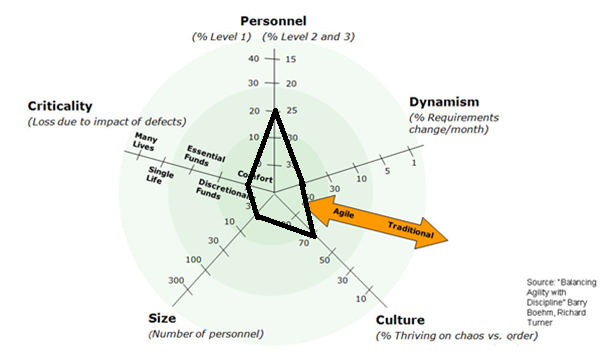
\includegraphics[scale=1.00]{includes/billeder/bohmsmodel.png}
\caption{Bohms model}
\label{fig:risici:bohms_model}
\end{center}
\end{figure}

\subsection*{Bohms model ~\ref{fig:risici:bohms_model}} 
Vi en lille gruppe p� 3, med kun 2 udviklere. Det er ikke kritisk om hvorvidt appen skulle crashe s� vi har vurderet Criticality til Comfort. For Personnel har vi vurderet til at ligger cirka midt p� idet at vi har meget forskelligt fagligt niveau i forhold til kodning. Vi forventer at der bliver brug for meget dynamik, idet at vi har lidt kendskab til teknologierne og at der derfor h�jst sandsynligt vil opst� en masse �ndringer undervejs i processen. I gruppen trives vi med en lille smule overordnet planl�gning, men ellers p� kaos og h�j personlig frihed.

\subsection*{Risici analyse}
Vi har valgt at fokusere p� risici for Android og Windows mobile idet at vi mener at disse er blandt de mest relevante teknologier i forhold til vores app. Yderligere kunne man evt. vurdere for IPhone og mobile web.

\subsubsection*{Android mobile}
\begin{figure}[H]
\begin{center}
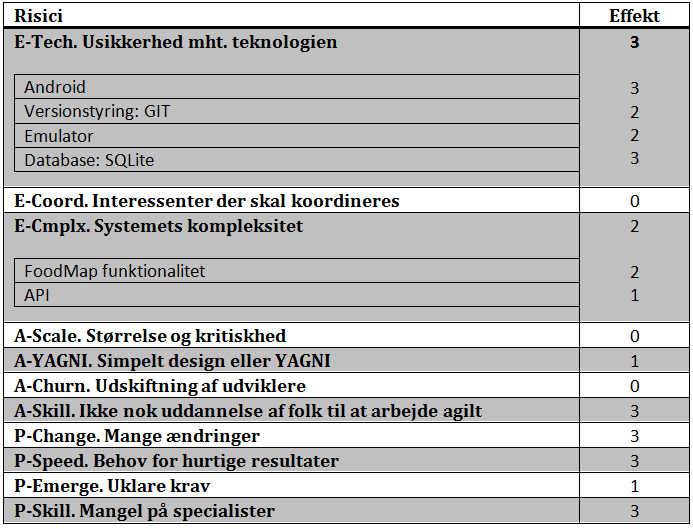
\includegraphics[scale=0.70]{includes/billeder/risici_analyse_android.png}
\caption{Risici analyse android}
\label{fig:risici:analyse_android}
\end{center}
\end{figure}

\textsf{Omgivelser (Enviroment):} ~\ref{fig:risici:analyse_android} \\
Vi har vurderet at der er h�j usikkerhed mht. teknologien specielt ift. Android og SQLite. Der er ikke nogen interessenter der skal koordineres. Systemets kompleksitet vil have en moderat effekt, mest er det FoodMap funktionaliteten som kan vise sig problematisk da vi ikke helt ved hvad den indeb�rer, samt at der vil forekomme nogle performance og usability krav der hurtigt kan g�re systemet komplekst. \\ 
\textsf{E-risici ialt:} 3 + 0 + 2 = 5
\\ \\


\textsf{Agile A-risici:} ~\ref{fig:risici:analyse_android} \\
Umiddelbart er det er et relativt sm�t projekt, derfor har vi vurderet A-Scale til ikke at have nogen effekt. Simpelt design vil ikke have den store effekt, da der ikke beh�ves den store planl�gning eller dokumentation af systemet. Der vil ikke v�re nogen udskiftning af udviklere s� A-Churn har ingen effekt. A-Skill kan g� hen at f� en stor effekt, idet at vores uddannelsesniveau er meget lavt i forhold til teknologien. \\ \\    
\textsf{A-risici ialt:} 0 + 1 + 0 + 3 = 4 \\ \\

\textsf{Plan-driven P-risks:} ~\ref{fig:risici:analyse_android} \\
Vi forventer at der vil forekomme mange �ndringer og dette vil have en stor effekt. Derudover er der et behov for hurtige resultater, idet at vi har brug for l�bende releases for at f� feedback fra reviews. Uklare krav vil have en meget lille effekt, idet at det i h�j grad er os selv der definerer dem. Mangel p� specialister vil have en stor effekt, da specialiser er n�dvendige for at kunne bruge de plandrevne v�rkt�jer ordentligt med den p�g�ldende teknologi. \\
\textsf{P-risici ialt:} 3 + 3 + 1 + 3 = 10

\newpage

\subsubsection*{Windows mobile} 
\begin{figure}[H]
\begin{center}
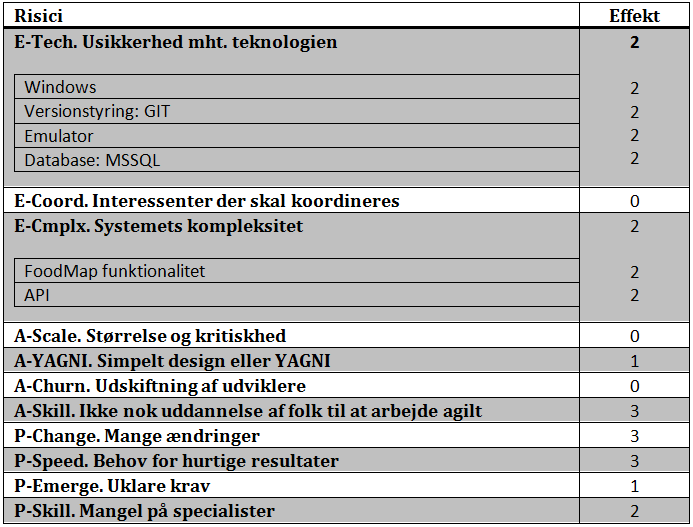
\includegraphics[scale=0.70]{includes/billeder/risici_analyse_windowsphone.png}
\caption{Risici analyse windowsphone}
\label{fig:risici:analyse_windowsphone}
\end{center}
\end{figure}

\textsf{Omgivelser (Enviroment):} ~\ref{fig:risici:analyse_windowsphone} \\
Vi har vurderet at der er j�vn usikkerhed mht. teknologien idet at vi ikke den store viden for Windows mobile, dog har vi tidligere erfaring med Visual studio og MSSQL. Der er ikke nogen interessenter der skal koordineres. Systemets kompleksitet vil have en moderat effekt, mest er det FoodMap funktionaliteten som kan vise sig problematisk da vi ikke helt ved hvad den indeb�rer, samt at der vil forekomme nogle performance og usability krav der hurtigt kan g�re systemet komplekst. \\ \\
\textsf{Enviroment effekt ialt:} \\
2 + 0 + 2 = 4 \\ \\

\textsf{Agile A-risici} og \textsf{Plan-driven P-risks:} ~\ref{fig:risici:analyse_windowsphone} \\
Umiddelbart er vilk�rene de samme som for Android mobile, men idet at vi har arbejdet mere med .NET, Visual studio og MSSQL forinden har vi valgt at vurdere effekten p� P-Skill lavere. \\
\textsf{A-risici ialt:} \\
0 + 1 + 0 + 3 = 4 \\

\textsf{P-risks ialt:} \\
3 + 3 + 1 + 2 = 9

\section*{Metodevalg}
Da vi er en lille gruppe som har det bedst med at der ikke er en for stram process og meget personlig frihed under ansvar, foretr�kker vi en meget agil udviklingsmetode og process. \\
Man m� ud fra vores risici-analyse konkludere at vi har meget usikkerhed med teknologien og at det derfor vil v�re en god ide at s�rge for at f� noget kvalitetssikring ind over udviklingen, gerne i form af unit testing.
Det ser umiddelbart ud som om at Windows mobile er nemmere at tilg�, men idet at Android markedet har flere brugere, finder vi det mere relevant at arbejde med.

\newpage

\section*{Projektplanl�gning og styring}
Til planl�gning og styring benytter vi iterationsplan med userstories og tasks samt releaseplan og burndown chart.

\subsection*{Kvalitetssikring og test}
Vi benytter pair programming i det omfang det ellers giver mening. \\
I det f�rste 3 sprints har vi valgt ikke at benytte unit testing da vi i forvejen, p� grund af teknologien, er pressede tidsm�ssigt til at have funktionalitet f�rdigt til produkt reviews. \\ 
Continuous integration ville blive for tidskr�vende at s�tte op. 

\subsection*{Deployment og konfigurationsstyring}
Det t�tteste vi kommer p� deployment er at teste appen p� en tablet.

\newpage

\subsection*{Velocity}
Vi forventer at have 4 timer om dagen per mand i gruppen. Dvs. 8 mandetimer om dagen med 2 hold. \\
4 dage f�rste uge. \\
4 dage anden uge. \\
3 dage tredje uge. \\

5 storypoint (standard) tager 8 mandetimer \\
5/8 = 0,625 storypoint per mandetime \\

%dette skal �ndres...
40 mande timer i en iteration
40*0,625 = 25 storypoints per uge
			5 storypoints per dag \\

4 sprints i alt.

\subsection*{Revurderet Velocity}
F�lgende har vi fundet ud af vores velocity er lavere pga. manglende erfaring og teknisk niveau for nogle i gruppen.
Dette resulterer i at vi ikke helt har resourcerne for to hold men n�rmere 1,5.\\

Vi forventer at have 4 timer om dagen per mand i gruppen. Dvs. 6 mandetimer om dagen med 1,5 hold.\\

24 mande timer i en iteration\\
24*0,625 = 15 storypoints per uge\\
			3,75 storypoints per dag \\

\newpage

\section*{Sprint 0}
Sprint 0 benyttede vi til at lave produktbacklog, iterationsplan og burndown. Samt at lave spike p� interfacet til foodmappet. \\
Vi skulle ogs� have lavet spike p� database men n�ede det ikke. \\ 
I �vrigt var Bjarke var ikke tilstede hverken onsdag, torsdag og fredag pga. Gr�n IT.

\newpage

\section*{Sprint 1 med XP}
\subsection*{Velocity}
I sprint 1 forventede vi at have 4 timer om dagen per mand i gruppen. Dvs. 8 mandetimer om dagen med 2 hold med
4 arbejdsdage. \\
Vi regnede os til at 5 storypoint (standard) tager 8 mandetimer \\
Det svarer til: 5 storypoints / 8 mandetimer = 0,625 storypoint per mandetime \\

32 mande timer i en iteration. \\
32 mandetimer * 0,625 = 20 storypoints per uge, dvs. 5 storypoints per dag. Dog tog vi et ekstra storypoint med for ugen.

\subsection*{Planl�gning}
Til sprintet afbillede vi vores burndown som en funktion af storypoints per mandedage. \\

% inds�t burndown her
%

I sprintet fokuserede vi p� 2 userstories:
\begin{itemize}
\item Kunden vil gerne have flere forslag til ingredienser frem p� food map, ved at trykke p� den midterste knap.
\item Kunden vil gerne have adgang til database.
\end{itemize}

I disse userstories omhandlede tasks med: 
\begin{itemize}
\item database design
\item oprettelse af tabeller
\item gui samt generel funktionalitet til foodmap
\end{itemize}


Backloggen s� i sprint 1 s�dan ud:
%link til at genere tabeller: http://www.tablesgenerator.com/
\begin{table}[h]
\begin{tabular}{llll}
Userstory                                                                                                                                                                    & \begin{tabular}[c]{@{}c@{}}Story-\\ points\end{tabular} & \begin{tabular}[c]{@{}c@{}}Mande-\\ timer\end{tabular} & Prioritet                \\ \hline
\multicolumn{1}{|l}{\begin{tabular}[c]{@{}c@{}}Kunden vil gerne have flere forslag til\\ ingredienser frem p� food map, ved at\\ trykke p� den midterste knap.\end{tabular}} & \multicolumn{1}{|l}{3}                                  & \multicolumn{1}{|l}{3}                                 & \multicolumn{1}{|l|}{1}  \\ \hline
\multicolumn{1}{|l}{\begin{tabular}[c]{@{}c@{}}Kunden vil have et animeret foodmap, \\ hvor ingredienser popper ud fra den\\ eksisterende ingrediensbobbel.\end{tabular}}    & \multicolumn{1}{|l}{}                                   & \multicolumn{1}{|l}{}                                  & \multicolumn{1}{|l|}{2}  \\ \hline
\multicolumn{1}{|l}{\begin{tabular}[c]{@{}c@{}}Kunden vil gerne kunne fjerne og tilf�je\\ ingredienser i food map.\end{tabular}}                                             & \multicolumn{1}{|l}{}                                   & \multicolumn{1}{|l}{}                                  & \multicolumn{1}{|l|}{3}  \\ \hline
\multicolumn{1}{|l}{\begin{tabular}[c]{@{}c@{}}Kunden vil gerne have en liste over forskellige\\ opskrifter som er udvalgt af \\ de anf�rte ingredienser.\end{tabular}}      & \multicolumn{1}{|l}{}                                   & \multicolumn{1}{|l}{}                                  & \multicolumn{1}{|l|}{4}  \\ \hline
\multicolumn{1}{|l}{\begin{tabular}[c]{@{}c@{}}Kunden vil gerne have hurtig s�geforslag \\ til ingredienser. (Performance)\end{tabular}}                                     & \multicolumn{1}{|l}{}                                   & \multicolumn{1}{|l}{}                                  & \multicolumn{1}{|l|}{5}  \\ \hline
\multicolumn{1}{|l}{\begin{tabular}[c]{@{}c@{}}Kunden vil gerne have listet opskrifter med\\ billeder, beskrivelse, ingredienser og \\ tilberedning.\end{tabular}}           & \multicolumn{1}{|l}{}                                   & \multicolumn{1}{|l}{}                                  & \multicolumn{1}{|l|}{6}  \\ \hline
\multicolumn{1}{|l}{\begin{tabular}[c]{@{}c@{}}Kunden vil gerne kunne f� et hurtigt overblik\\  over indk�bs- og pr�perationsliste ved opskrift.\end{tabular}}               & \multicolumn{1}{|l}{}                                   & \multicolumn{1}{|l}{}                                  & \multicolumn{1}{|l|}{7}  \\ \hline
\multicolumn{1}{|l}{\begin{tabular}[c]{@{}c@{}}Kunden vil gerne have en menu til navigering\\ i appen.\end{tabular}}                                                         & \multicolumn{1}{|l}{}                                   & \multicolumn{1}{|l}{}                                  & \multicolumn{1}{|l|}{8}  \\ \hline
\multicolumn{1}{|l}{\begin{tabular}[c]{@{}c@{}}Kunden vil gerne kunne gemme indk�bsliste\\ i indk�bsoversigt.\end{tabular}}                                                  & \multicolumn{1}{|l}{}                                   & \multicolumn{1}{|l}{}                                  & \multicolumn{1}{|l|}{9}  \\ \hline
\multicolumn{1}{|l}{\begin{tabular}[c]{@{}c@{}}Kunden vil gerne kunne gemme opskrifter i\\ favoritter.\end{tabular}}                                                         & \multicolumn{1}{|l}{}                                   & \multicolumn{1}{|l}{}                                  & \multicolumn{1}{|l|}{10} \\ \hline
\multicolumn{1}{|l}{\begin{tabular}[c]{@{}c@{}}Kunden vil gerne have en s�rskilt indk�bsliste,\\  som kan tilg�s fra hovedmenuen.\end{tabular}}                              & \multicolumn{1}{|l}{}                                   & \multicolumn{1}{|l}{}                                  & \multicolumn{1}{|l|}{11} \\ \hline
\end{tabular}
\end{table}

\subsection*{Xp praktikker}
I sprint 1 benyttede vi XP praktikkerne: planning poker, par programmering, kollektivt kode ejerskab, refactoring, kodestandarder, metafor og simpelt design. \\

Vi lavede planning poker med storypoints til at vurdere st�rrelsen af userstories for senere hen at udregne vores velocity. \\
Vi arbejdede med par programmering i 2 grupper, hvor vi ogs� i h�j grad havde den af grupperne med en mand i til at unders�ge teknologien. Vi fors�gte s� vidt muligt at f� alle ind over koden hvor vi i forvejen havde aftalt at bruge Java camelcasing samt at refactorer koden med KISS som m�l.
Derudover vi benyttede dom�ne model og database schema til design for at f� enighed om samt overblik over dom�net. 

Mht. kvalitetssikring valgte vi ikke at benytte test-first eller unit testing eftersom vi p� dette tidspunkt ikke rigtigt havde noget relevant at teste p� samt at vi prioriterede funktionalitet.


\subsection{Produkt review}
Til reviewet i starten af sprint 2 pr�senterede vi vores grafiske brugergr�nseflade: 
% inds�t screenshot her.
 
\subsubsection*{Konklusion af review}
At vi havde et lovende interface med statisk funktionalitet, men uden database adgang.


\subsection*{Retrospektive}
Vi l�b ind i et problem med at vores userstory for databasen, hvilken var for bredt defineret. Dette resulterede i at vi ikke kunne tegne vores burndown ned overhovedet. 

\subsubsection*{Ting der gik godt}
Par programmering \\
Kollektivt kode ejerskab.



\subsubsection*{Mindre godt}
Vores opsplitning af user stories: \\
Vores user stories skal splittes mere og bedre op, s� vi er istand til at tegne burndown ned.
Burndown som er sammensat ved point og dage.
skriv logbog hver dag.
Korrigere for frav�r.


Andet
Vi lavede ikke test-first - Dette var ikke muligt da vi ikke er erfarne med android

Ting vi forts�tter med
Vi forts�tter med pair-progamming til de mere komplekse tasks

Ting vi vil forbedre
Burndown sammensat af timer og dage, i stedet for point.
Opdeling af user stories
Vil lave burndown af tasks istedet for user stories
Vores accept tests.

\newpage

\subsection*{Sprint 2}
Ud fra sprint 1 har vi erfaret at for store user stories giver en uklar pr�sentation af fremskridt p� vores burndown. Vi startede s�ledes sprint 2 med at dele nogle af vores user stories op. Herefter lavede vi planning poker for at f� et mere n�jagtigt estimat af hvor lang tid de forskellige stories ville tage. Endvidere, for samtidigt at f� et mere n�jagtigt burndown, begyndte vi at br�nde det ned i mandetimer fremfor user stories, samt s�tte mandetimer p� de enkelte tasks.
Sprintet 2 handlede i h�j grad om at lave user stories for database samt koblingen mellem databasen og foodmap.

\subsection*{Velocity}
Vi har ikke �ndret p� vores velocity fra sprint 1, da vi mener at vi ikke fik br�ndt ned p� burndown pga. for store user stories og d�rlig estimering. Vi forventede derfor at have 4 mandetimer om dagen per mand i gruppen. Dvs. 8 mandetimer om dagen med 2 hold med 4 arbejdsdage. \\
Story points og mandetimer forblev det samme som i sprint 1: 5 story points pr 8 mandetimer, 0,625 story points per mandetime, 32 mande timer i sprintet og 20 story points per uge, dvs. 5 story points per dag.

\subsection*{Planl�gning}
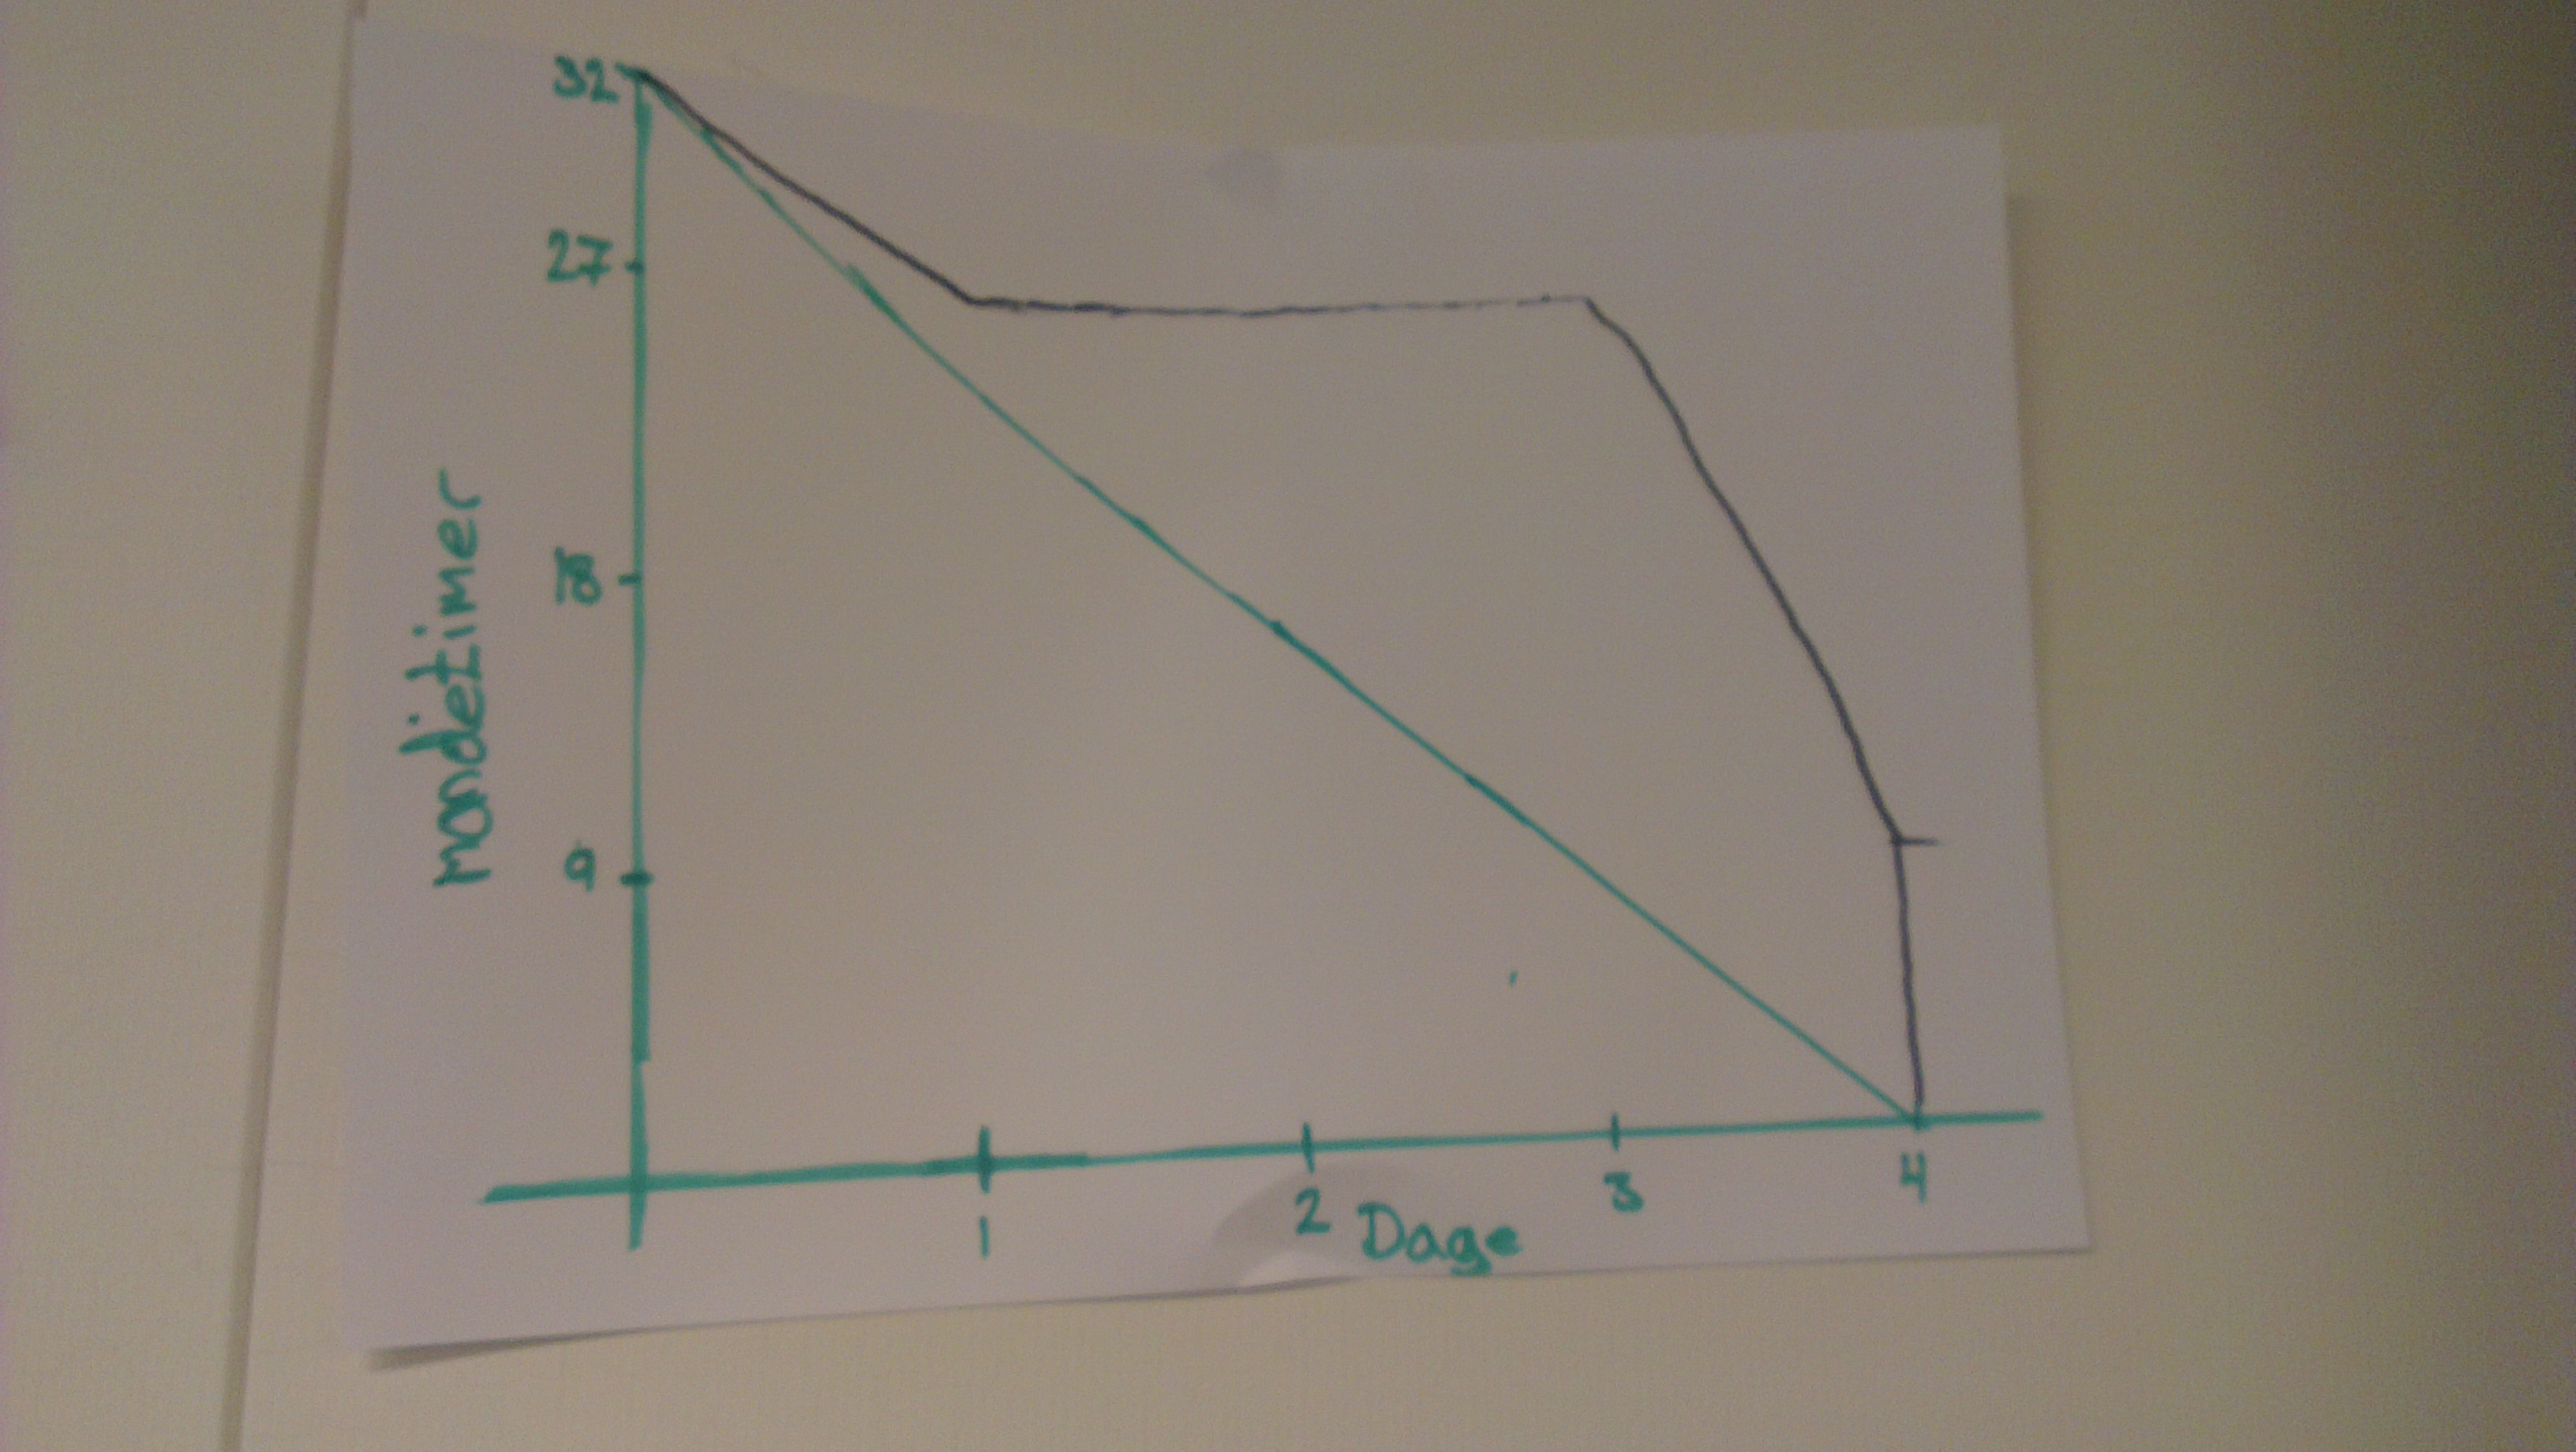
\includegraphics[scale=0.10]{includes/billeder/sprint2.jpg}
\subsubsection*{Product backlog}
Backlog lavet den 9.12.2013 i starten af sprint 2. \\
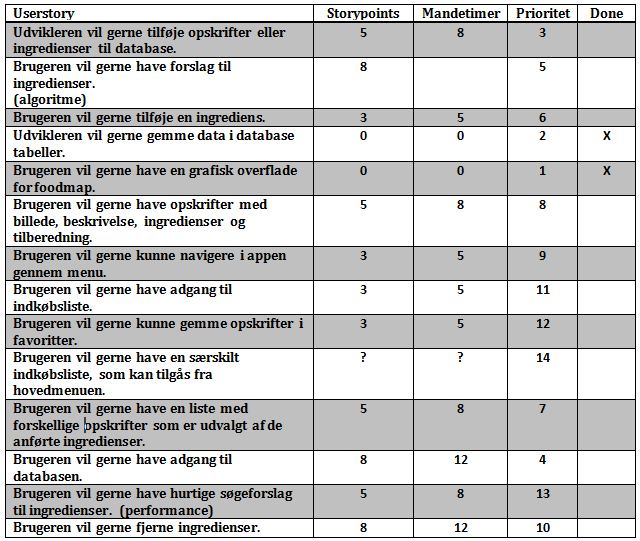
\includegraphics[scale=0.60]{includes/billeder/productbacklog_sprint2.png}

\subsubsection*{Sprint backlog}
I sprint 2 fokuserede vi p� f�lgende user stories: \\
Database kobling, dummy data til databasen, algoritme. \\
Samt database tabeller og basic gui som vi satte til 0 mandetimer, eftersom de var f�rdige efter at have opdelt dem, da de var for store. 

\subsection*{Xp og scrum praktikker}
I sprint 2 benyttede vi XP praktikkerne: stand-up meeting, planning poker, par programmering, kollektivt kode ejerskab, refactoring, kodestandarder, metafor og simpelt design. \\
Vi havde en scrum master, men product owner droppede vi, da det ikke giver s� meget mening i en gruppe af 3.

\subsection*{Produkt review}
Til produkt reviewet var det planen at vi ville vise vores gui med database adgang, men Android emuleratoren fejlede og pr�sentationen faldt derfor til bunden. Det endte med at vi kun viste selve databasen med data. 


\subsection*{Retrospektive}
I sprint 2 blev vi endeligt f�rdige med b�de databasen og koblingen mellem database og gui, dog f�rst efter at have en del overarbejde. Samtidigt havde vi overvurderet hvor mange ressourcer vi egentligt havde til r�dighed og n�ede derfor at br�nde 20 ud af 32 mandetimer.

\subsubsection*{Hvad gik godt}
Sprint 2 gik meget bedre end sprint 1 idet at vi endeligt fik styr p� database delen af vores projekt, dog efter meget overarbejde. Samtidigt fik vi en positiv oplevelse af at f� opsplittet vores user stories bedre, da de dermed blev mere pr�cise b�de i formulering og estimering. 

\subsubsection*{Hvad gik mindre godt}
Vi skulle have v�ret lidt bedre forberedt til produkt reviewet; det kunne m�ske have v�ret muligt at undg� problemer med emulatoren og kunden havde f�et et bedre indtryk af hvad vi havde lavet.

\subsubsection*{Hvad �ndrer vi til n�ste sprint}
En revurdering af vores velocity, da vi �benlyst havde vurderet den for h�jt igen og m�tte s�ge at lave et mere overkommeligt m�l.

\newpage
\subsection*{Sprint 3}
\subsection*{Velocity}
Lav velocity blah blah...

\subsection*{Planl�gning}

\subsubsection*{Product backlog}
Til product backloggen har vi i dette sprint tilf�jet en userstory med unit testing, samt at vi har �ndret prioriteten for diverse stories. \\
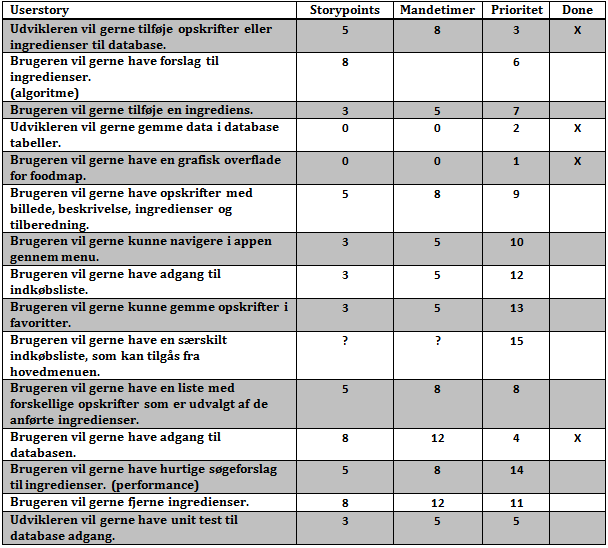
\includegraphics[scale=0.70]{includes/billeder/productbacklog_sprint3.png}

\subsubsection*{Sprint backlog}
I sprint backloggen for dette sprint indg�r de to userstories: \\
\begin{itemize}
\item Udvikleren vil gerne have unit test til database adgang.
\item Brugeren vil gerne have forslag til ingredienser. (algoritme)
\end{itemize}

Ud af disse to stories fik vi lavet unit testene.

\subsection*{Xp og scrum praktikker}
I sprint 3 benyttede vi fortsat XP praktikkerne: stand-up meeting, planning poker, par programmering, kollektivt kode ejerskab, kodestandarder, story board, metafor og simpelt design.

\subsection*{Produkt review}
Til reviewet viste vi vores foodmap gui med den funktionalitet vi havde n�et, samt vores unit test.

\subsubsection*{Konklusion af review}
N�ede kun unit testing.

\subsection*{Retrospektive}
Godt: \\
Vi fik lavet unit test og dermed fik vi lidt mere kvalitetssikring ind over vores projekt. \\

Kunne have v�ret bedre: \\
Alt for kort sprint med de 3 mandedage og derfor for meget pres p� for at have noget klar til reviewet. Is�r iforhold til at have noget visuelt klar at kunne vise. \\
Vi havde lidt meget parprogrammering pga. vores fokus p� test. 

Hvad �ndrer vi til n�ste sprint: \\
Vi var sprint 3 det sidste sprint, men ellers havde vi prim�rt fors�ge at lave et l�ngere sprint hvor vi arbejdede lidt mere spredt.




\section*{Konklusion p� sprints}

